\chapter{تست و بررسی سامانه}

بعد از فصل پیاده‌سازی، این فصل به تست و بررسی سامانه می‌پردازد. برای تست سامانه، موارد آزمون\LTRfootnote{\lr{Test case}} برای دو دسته نیازمندی‌های کارکردی و غیرکارکردی نوشته شده و هریک به صورت جداگانه بررسی می‌شود. اما در بعضی موارد به دلیل فرصت کم به بررسی نیازمندی‌ سامانه بسنده می‌شود. شرایط تست و بررسی نیازمندی‌های مختلف نیز به صورت زیر است:
\begin{itemize}
    \item نوع پردازنده مرکزی\LTRfootnote{\lr{Central Processing Unit (CPU)}} سیستم‌ها از نوع \lr{Intel(R) Core(TM) i7-10750H CPU @ 2.60GHz} است.
    \item سیستم شامل سامانه پایش شبکه و سیستم‌های دیگر جهت تست کشف شبکه، هر کدام دارای دو هسته مجازی هستند.
    \item سیستم شامل سامانه پایش شبکه دارای چهار گیگابایت حافظه اصلی\LTRfootnote{\lr{Random-access memory (RAM)}} و سیستم‌های دیگر جهت تست کشف شبکه، هر کدام دارای دو گیگابایت حافظه اصلی هستند.
\end{itemize}


در ادامه در بخش‌های تست نیازمندی‌های کارکردی و غیرکارکردی به موارد آزمون یا بررسی نیازمندی‌های مختلف پرداخته می‌شود.

\section{تست و بررسی نیازمندی‌های کارکردی}

\subsection{تست کشف شبکه}

برای تست کشف شبکه با استفاده از ماشین‌های مجازی\LTRfootnote{\lr{Virtual Machine (VM)}} و سوئیچ‌های مجازی\LTRfootnote{\lr{Virtual Switch}}، برای دو سناریو مورد آزمون تولید شد. به عبارتی دو شبکه طبق \cref{fig.51} و \cref{fig.52} طراحی شد. سپس با استفاده از قابلیت کشف شبکه سامانه خروجی این دو سناریو دریافت شد، که در \cref{fig.511} و \cref{fig.521} قابل مشاهده است.



\begin{figure}[!h]
    \centering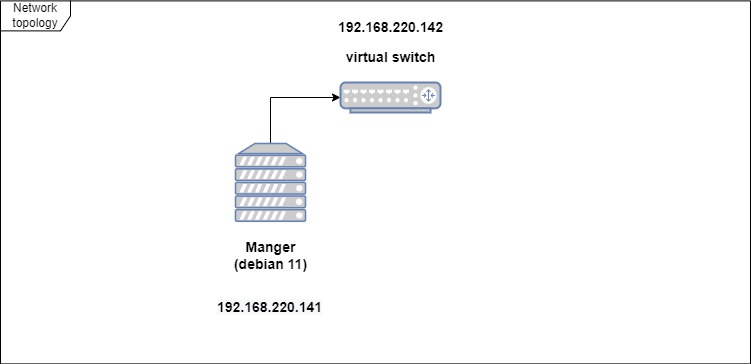
\includegraphics[scale=.55]{./topo-test1}
    \caption{تصویر توپولوژی شبکه اول جهت تست}\label{fig.51}
\end{figure}


\begin{figure}[!h]
    \centering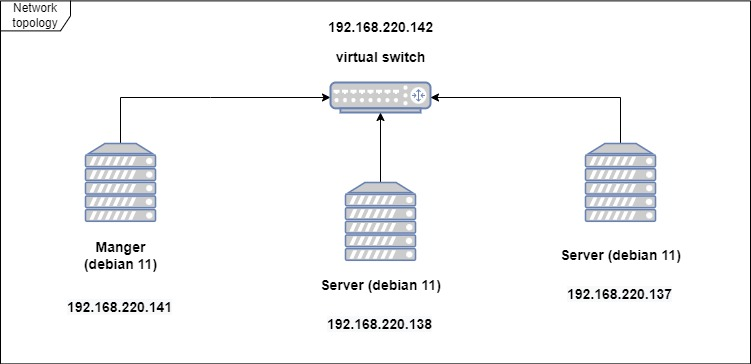
\includegraphics[scale=.55]{./topo-test2}
    \caption{تصویر توپولوژی شبکه دوم جهت تست}\label{fig.52}
\end{figure}


در \cref{fig.51} هدف پایش تنها یک دستگاه بود. در واقع با راه‌اندازی یک سیستم و سامانه پایش برروی همان سیستم، ماژول کشف شبکه سامانه باید بتواند خودش را به درستی شناسایی کند که این امر در \cref{fig.511} محقق می‌شود. 


\begin{figure}[!h]
    \centering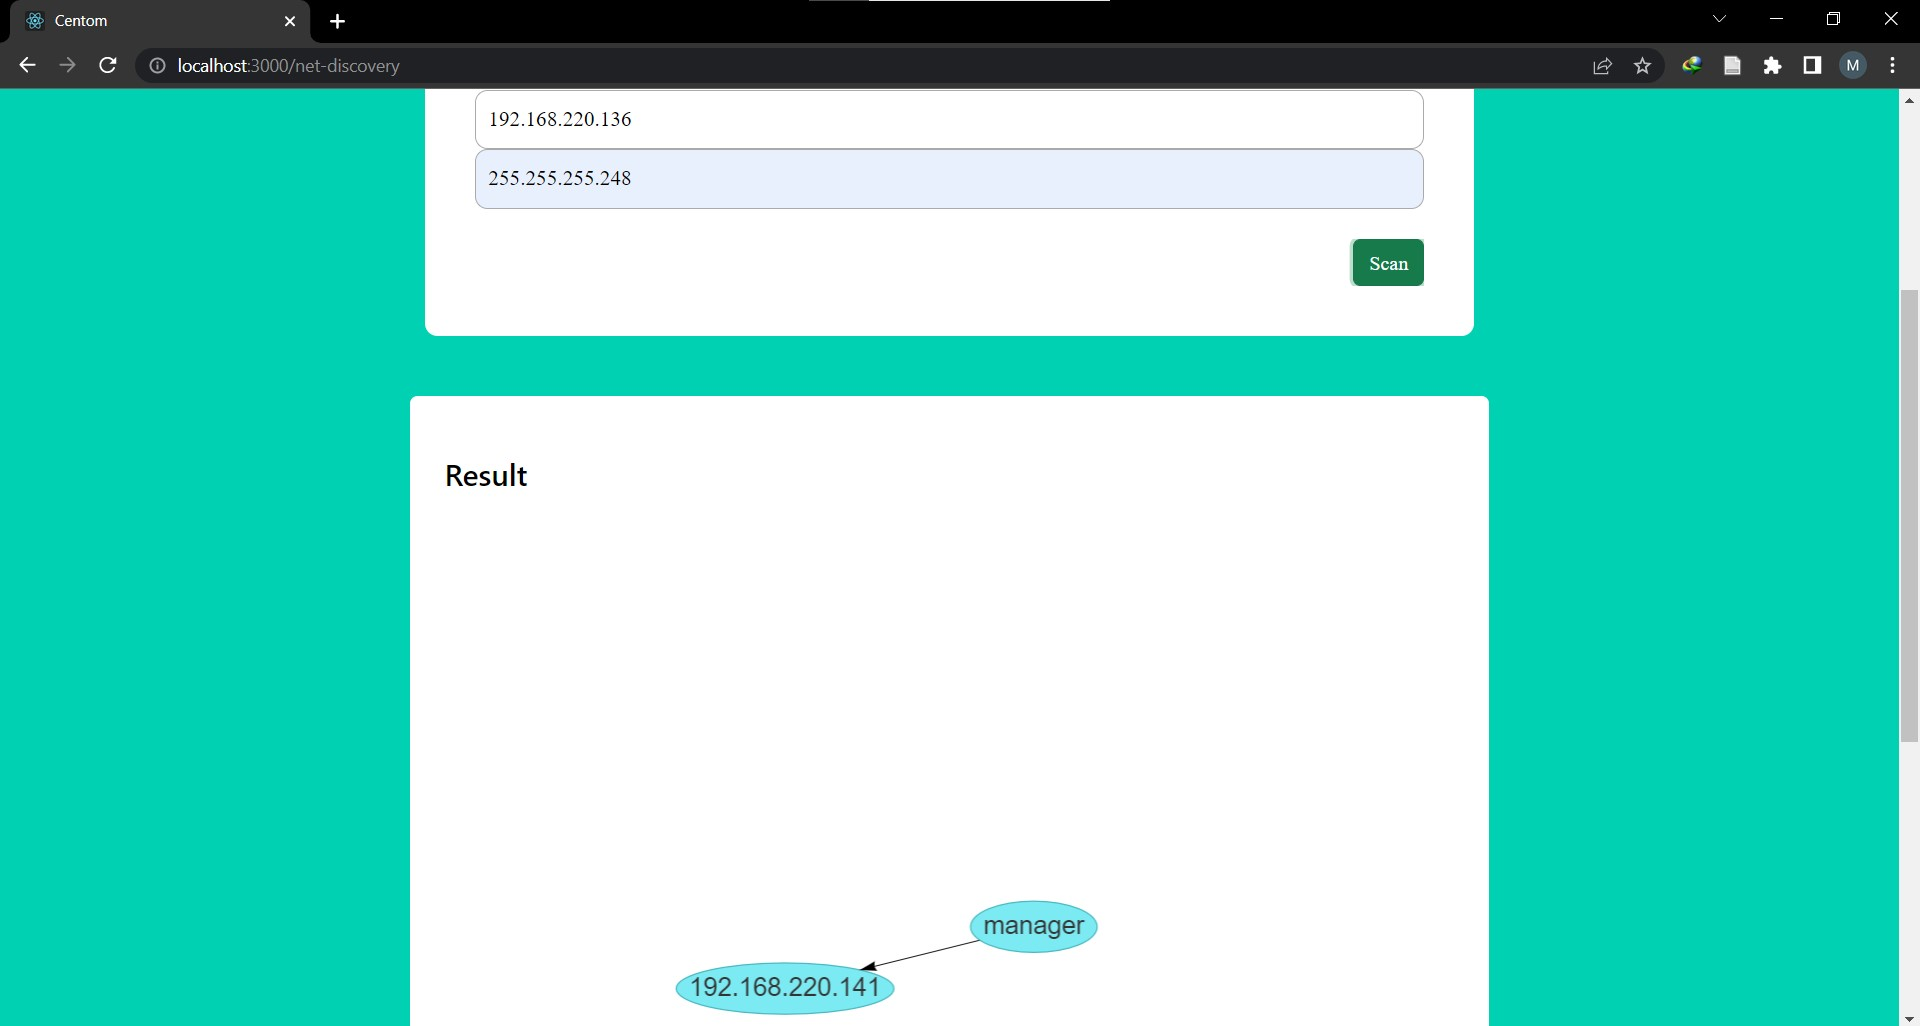
\includegraphics[scale=.38]{./topo-test1-result}
    \caption{تصویر توپولوژی بدست آمده برای شبکه اول}\label{fig.511}
\end{figure}


\begin{figure}[!h]
    \centering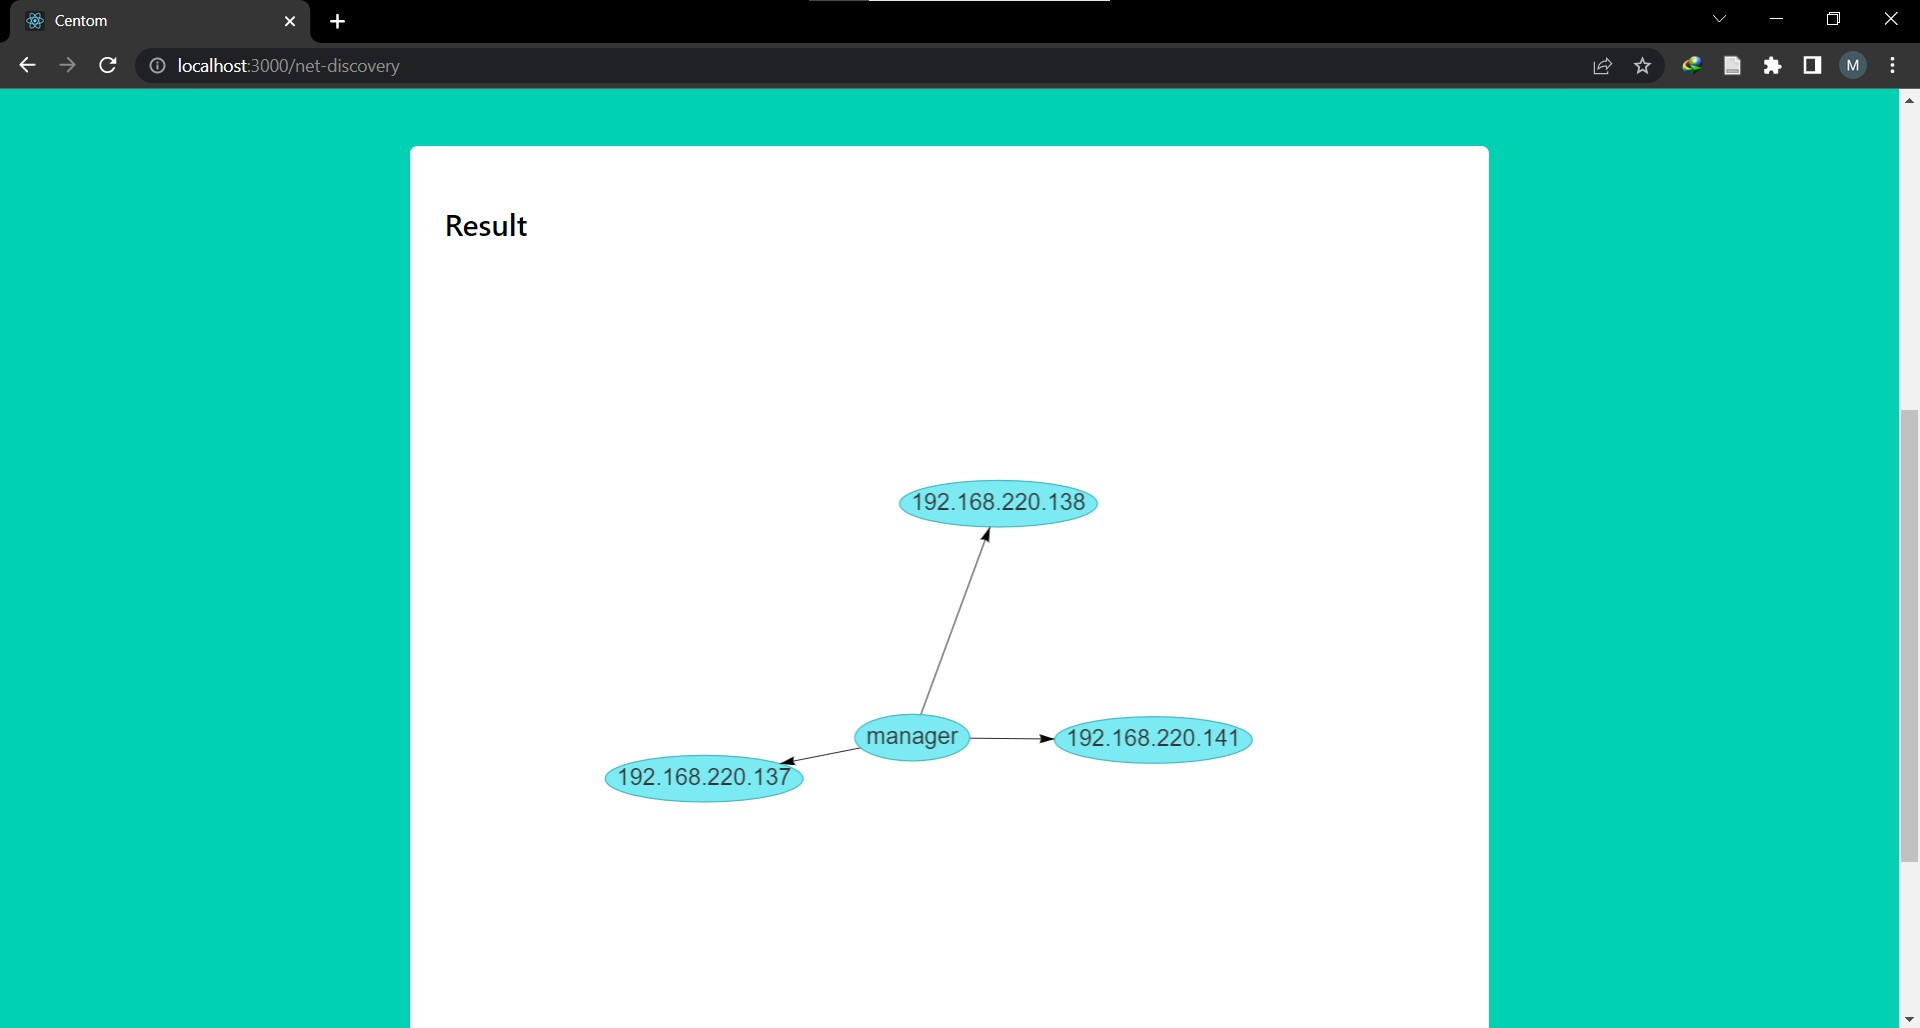
\includegraphics[scale=.38]{./topo-test2-result}
    \caption{تصویر توپولوژی بدست آمده برای شبکه دوم}\label{fig.521}
\end{figure}


بعد از انجام تست اول، به سوئیچ موجود در شبکه اول دو دستگاه مشابه دستگاه موجود، به شبکه اضافه می‌شوند. بعد از گرفتن خروجی شبکه دوم، مشاهده و واضح می‌شود که سوئیچ موجود در شبکه‌ها در خروجی وجود ندارد، که این امر بدین علت است که از سوئیچ مجازی برای تست استفاده شده است. خروجی شبکه دوم نیز در \cref{fig.521} نیز قابل مشاهده است که با شبکه طراحی شده مطابقت می‌نماید.


\cleardoublepage


\subsection{تست تنظیمات شبکه}

برای این بخش امکانی فراهم شده تا کاربر هنگام پایش اطلاعات شبکه، مواردی که در بخش تنظیمات ذخیره کرده است را مشاهده می‌کند. بدین صورت که کاربر ابتدا باید در صفحه پایش، تنظیمات دستگاه موردنظر را واکشی کند تا از صحت آن مطمئن شود. موارد بسیار زیادی در این بخش تست شد که به عنوان نمونه می‌توان به \cref{fig.18} اشاره کرد.


\subsection{تست پردازش و ذخیره اطلاعات جمع‌آوری شده}

این تست از دو بخش تشکیل می‌شود:

\begin{itemize}
    \item نمایش نمودارهای پایش عملکرد عنصر تحت مدیریت
    \item نمایش اطلاعات قدیمی در صورت پایش قبلی
\end{itemize}

برای بخش اول \cref{fig.53} کفایت می‌کند، چون نمودارها به صورت بی‌درنگ درحال نمایش اطلاعات دریافتی هستند.


برای بخش دوم نیز دوباره بعد از بستن صفحه موردنظر دوباره اقدام به پایش کرده که نتیجه آن در \cref{fig.54} قابل مشاهده است. درواقع اطلاعات قدیمی از ردیس بازیابی شده و نمایش داده می‌شود. همانطور که در \cref{fig.54} دیده شد، پرش مربوط در نمودارهای ارسال و دریافت برای مدت زمانی است که پایشی صورت نگرفته است اما از طریق سیستم اطلاعات ارسال و دریافت شده است.

\begin{figure}[!h]
    \centering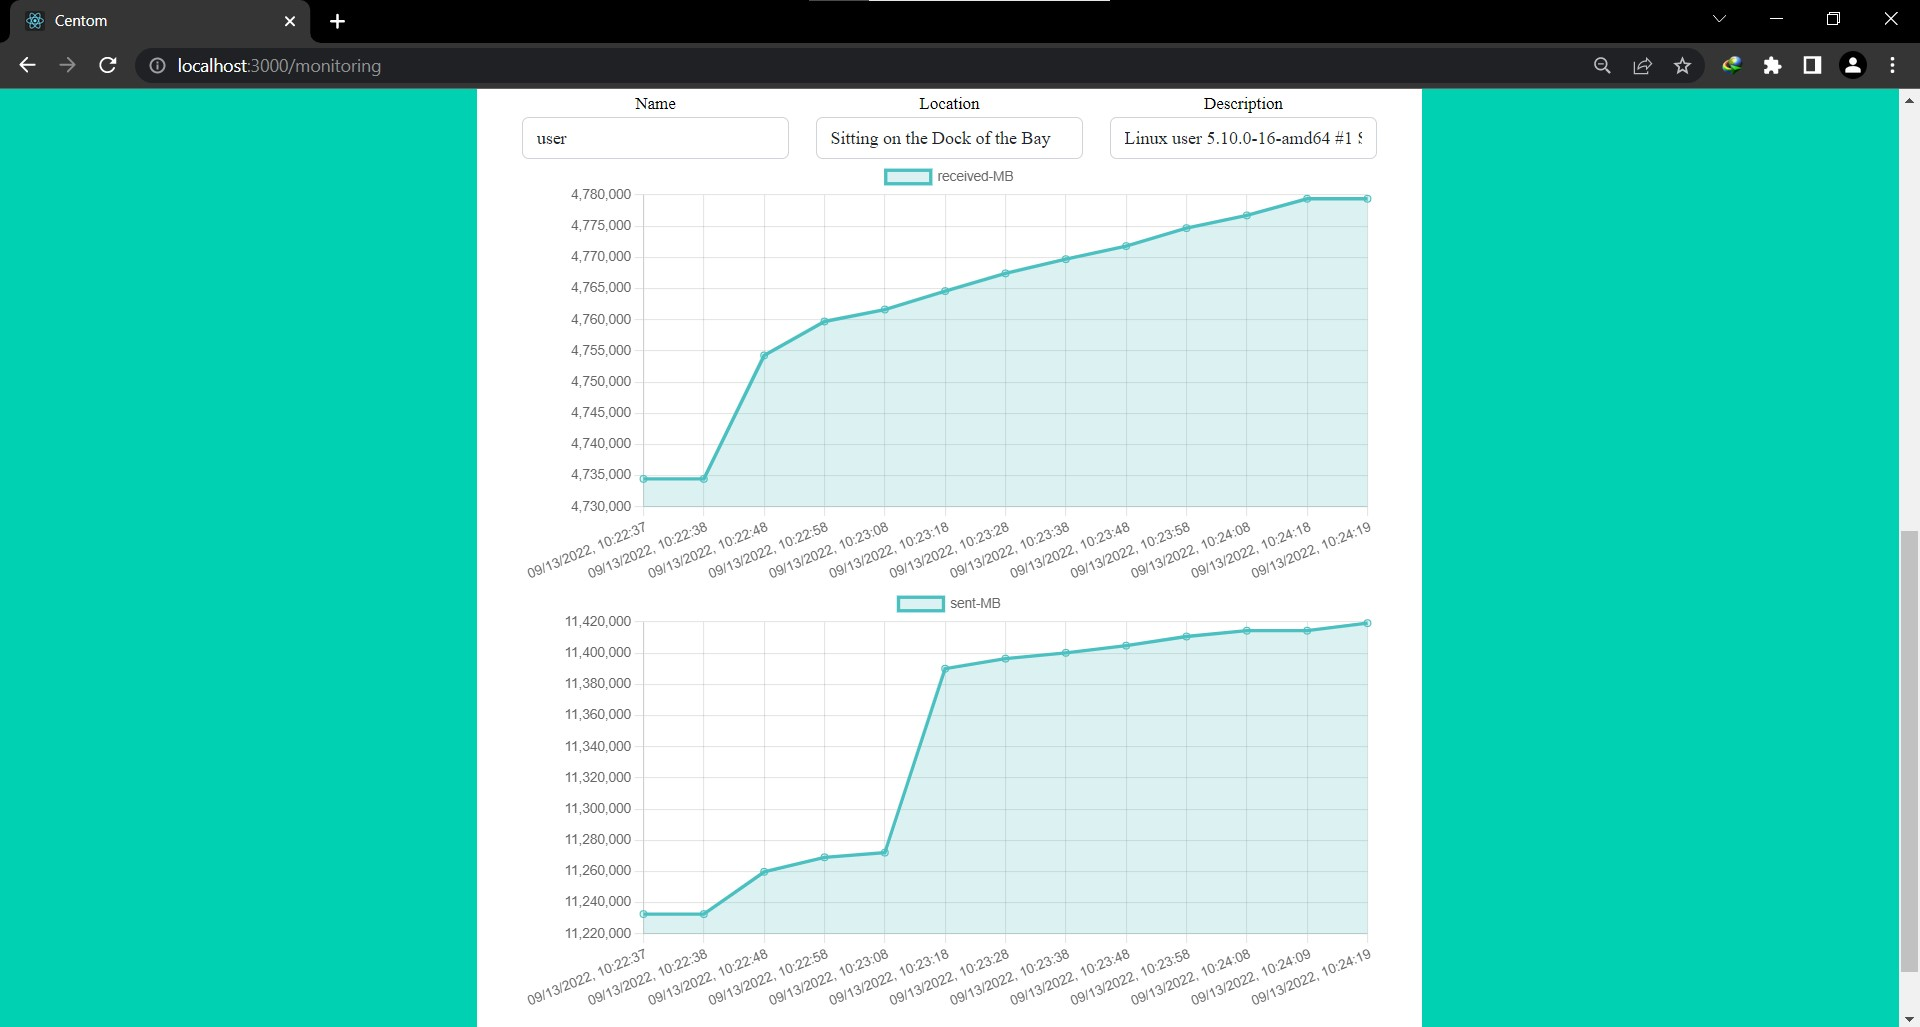
\includegraphics[scale=.38]{./monitoring-before}
    \caption{تصویر نمودارهای مربوط به پارامترها}\label{fig.53}
\end{figure}


\begin{figure}[!h]
    \centering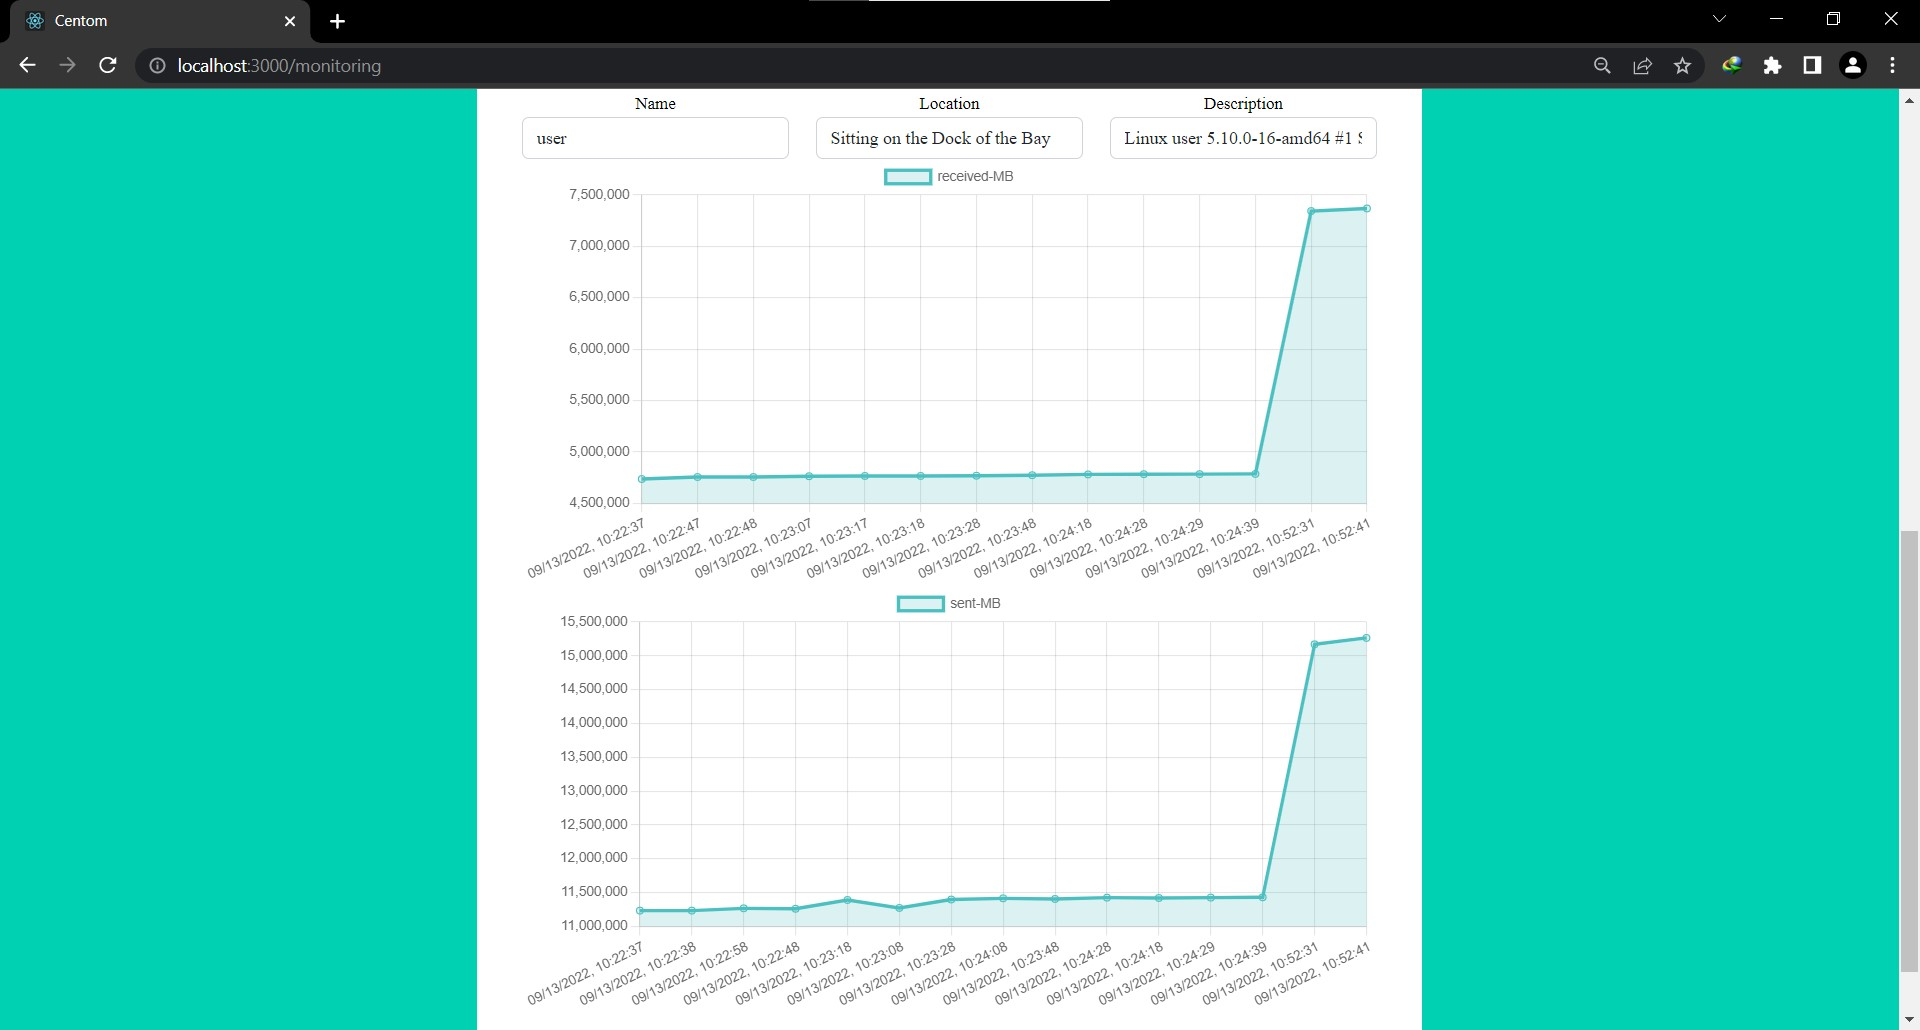
\includegraphics[scale=.38]{./monitoring-after}
    \caption{تصویر نمودارهای پارامترها جهت نمایش بازیابی صحیح اطلاعات}\label{fig.54}
\end{figure}



\cleardoublepage


\subsection{تست جمع‌آوری هشدارهای مربوط به عناصر تحت مدیریت}

برای این بخش از ابزار \lr{snmptrap} که تله‌ای مشخص می‌فرستد، استفاده شد. با این ابزار تله‌هایی طبق \cref{fig.55} به سامانه ارسال کرده و باید نتیجه در صفحه اعلانات بعد از فشردن دکمه مشاهده شود (به همان ترتیب و مقادیر)


همان‌طور که طبق \cref{fig.56} مشاهده می‌شود نتایج دقیقا با دستورات اجرایی مطابقت می‌نماید.


\begin{figure}[!h]
    \centering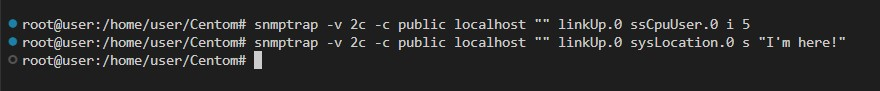
\includegraphics[scale=.70]{./trap-before}
    \caption{تصویر دستورات اجرا شده تله}\label{fig.55}
\end{figure}

\begin{figure}[!h]
    \centering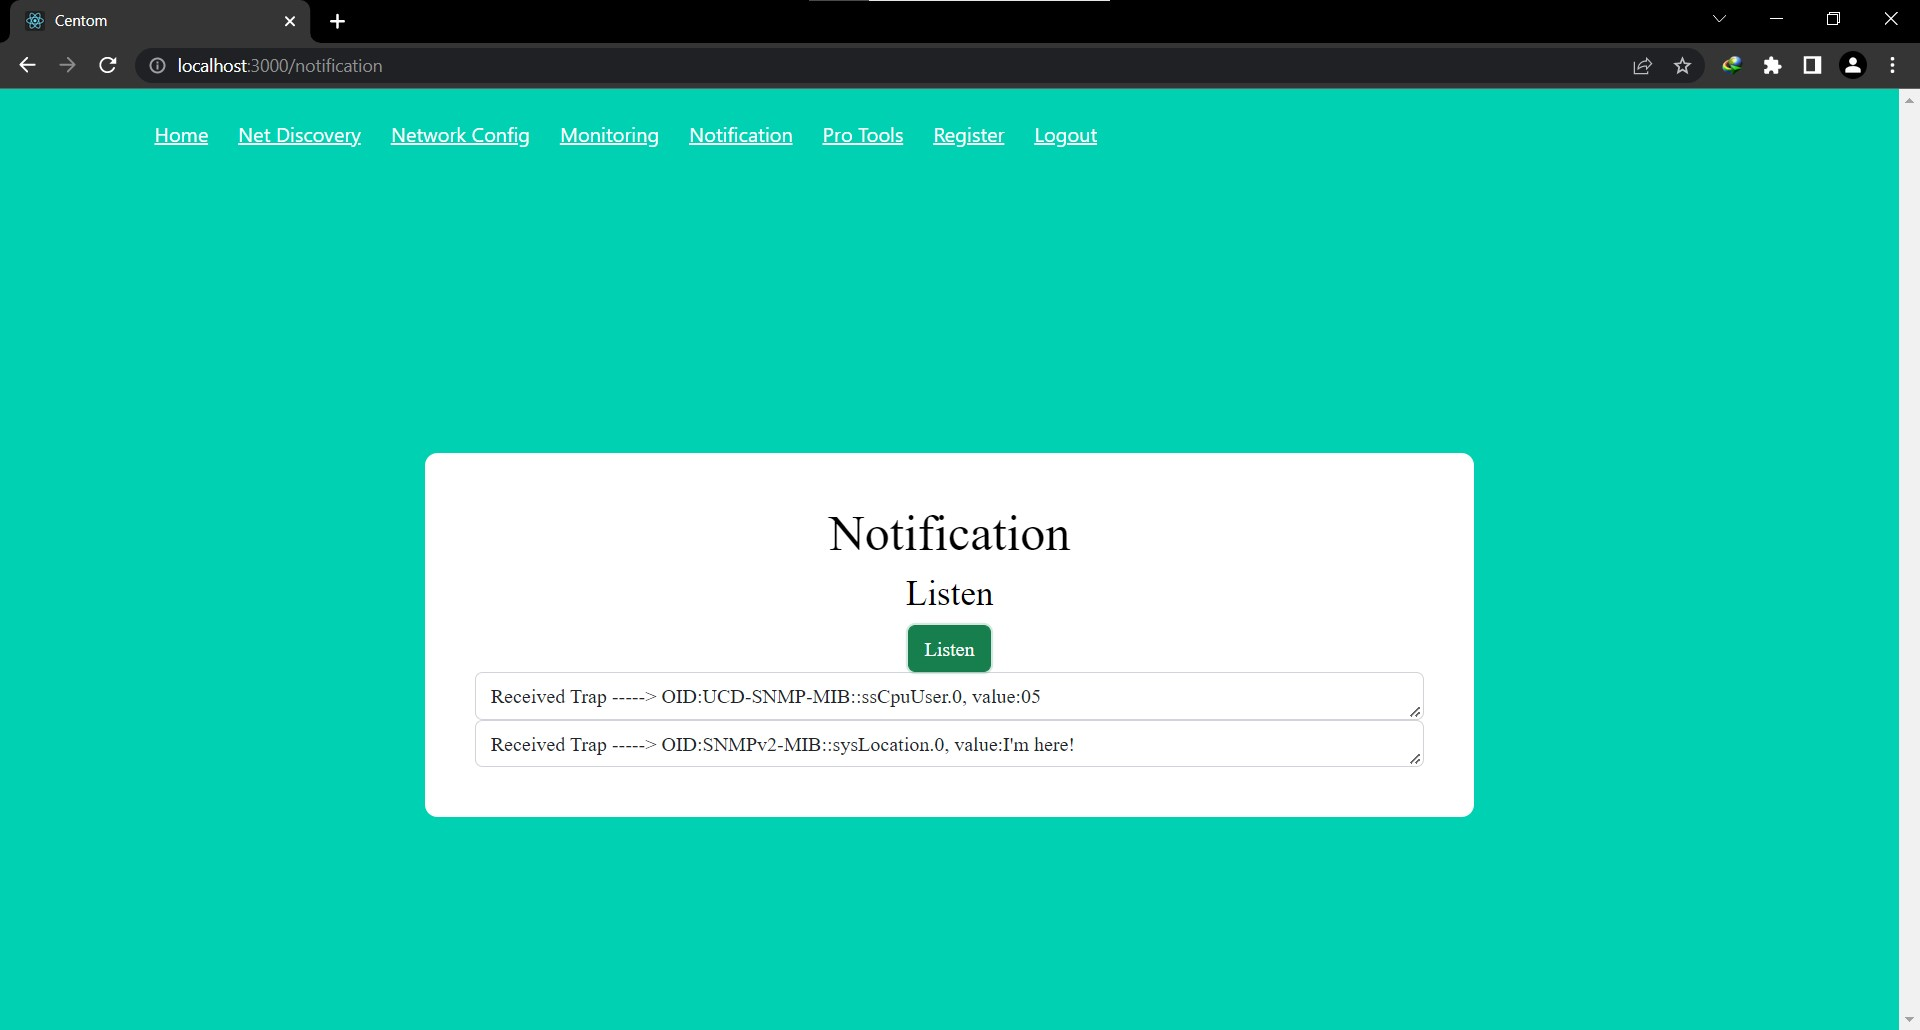
\includegraphics[scale=.38]{./notification}
    \caption{تصویر تله‌های دریافتی در سامانه}\label{fig.56}
\end{figure}

\cleardoublepage

\section{تست و بررسی نیازمندی‌های غیرکارکردی}


\subsection{تست مدت زمان کشف شبکه}

دقیقا همان تستی که در بخش نیازمندی‌های کارکردی برای تست کشف شبکه انجام شد، کیفیت (مدت زمان) آن در اینجا درنظر گرفته می‌شود. توجه شود که در هر دو سناریو آدرس شبکه 136.220.168.192 و همچنین نقاب زیرشبکه 248.255.255.255 در نظر گرفته شدند، که در سناریوی اول زمان کشف شبکه 35 ثانیه و در شبکه دوم 33 ثانیه بدست آمد. این اختلاف زمانی بدین خاطر است که در سناریوی اول زمان بیشتری جهت انتظار دریافت پیغام‌های \lr{SNMP} صرف شده است. البته این مقادیر کمتر از دو دقیقه (مقدار مطلوب) است.

\subsection{بررسی واسط کاربری مطلوب تحت وب}

پیاده‌سازی واسط کاربری این سامانه با چارچوب ری‌اکت و همچنین چارچوب فلسک در سمت سرور، رابط کاربری تحت وب مطلوبی را برای افراد فراهم می‌آورد. همچنین برای استفاده از سامانه بیرون از شبکه سازمان، با چند تغییر در تنظیمات شبکه می‌توان به آن دسترسی پیدا کرد. این رابط کاربری طبق بررسی‌های انجام شده و مشورت‌های صورت گرفته توسعه داده شده است. همچنین پرسشنامه‌ای جهت بررسی این نیازمندی در \cref{fig.57} طراحی شد ولی به دلیل فرصت کم امکان نظرسنجی از مدیران شبکه فراهم نشد.

\begin{figure}[!h]
    \centering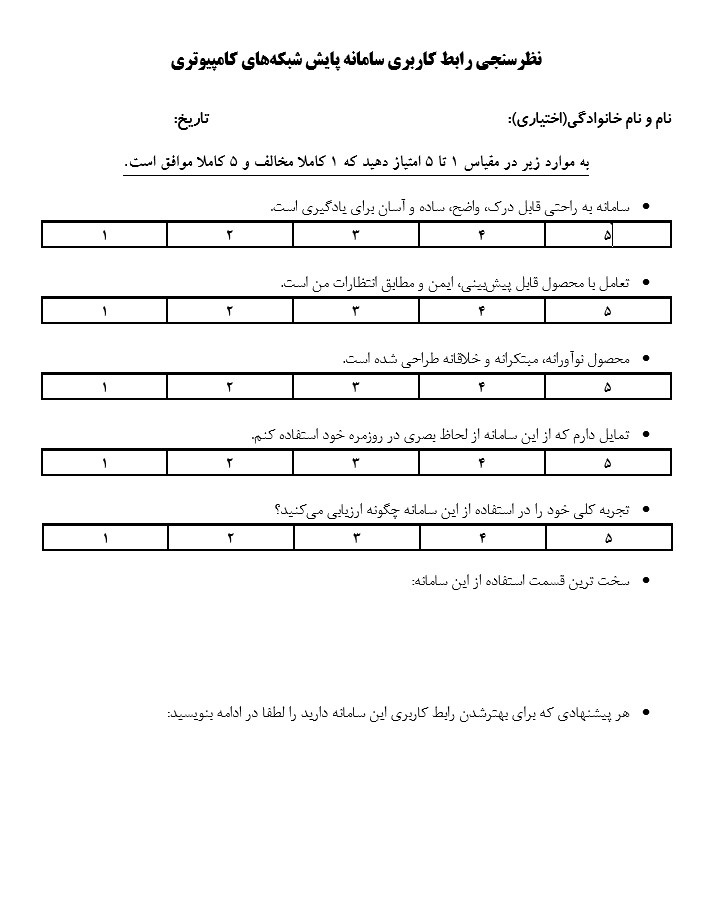
\includegraphics[scale=.90]{./survey}
    \caption{پرسشنامه طراحی شده برای بررسی واسط کاربری}\label{fig.57}
\end{figure}

\cleardoublepage

\subsection{بررسی امنیت سامانه}

این نیازمندی به دلیل فرصت کم تنها بررسی شد و تستی برای آن صورت نگرفت. امنیت سامانه باید از سه منظر محرمانگی، صحت و در دسترس بودن بررسی شود. در ادامه برای این بخش‌ها تدابیر صورت گرفته برای توسعه این سامانه ذکر می‌شوند.

\begin{itemize}
    \item برای فراهم آوردن محرمانگی داده‌ها از پروتکل \lr{SNMPv3} برای پایش اجزا استفاده شد که نیاز به نام کاربری و رمز عبور دارد.
    \item برای فراهم آوردن صحت داده‌ها استفاده از رمز عبور برای پایگاه‌های داده می‌تواند مفید باشد. به عنوان مثال برای ردیس رمز عبوری قوی بکار گرفته شد.
    \item در بحث در دسترس بودن سامانه کار ویژه‌ای انجام نشد، زیرا برای فراهم آوردن این ویژگی نیاز به یک فایروال در شبکه است تا به عنوان مثال از حملات منع دسترسی جلوگیری نماید. 
\end{itemize}